\documentclass[twocolumn]{article}
\usepackage{graphicx}
\usepackage{amsmath}
\usepackage{siunitx}
\usepackage{fancyhdr} 
\usepackage{fancybox}
\usepackage{float}
\usepackage{listings}
\usepackage[colorlinks=true,linkcolor=black]{hyperref}
%\usepackage[labelformat=empty]{caption}
\usepackage[margin=1.0in]{geometry}

\pagestyle{fancy}

%redefines subsections with letters instesad of numbers
\renewcommand{\thesubsection}{\thesection.\alph{subsection}}

% Center Image Command
\newcommand{\centerimage}[3]{
\begin{figure}[ht!]  
\begin{center}
#1
\caption{#2}
\label{#3}
\end{center}
\end{figure}}

\newcommand{\tstamp}{\today}   
%\renewcommand{\chaptermark}[1]{\markboth{#1}{}}
\renewcommand{\sectionmark}[1]{\markright{#1}}
\lhead[\fancyplain{}{\thepage}]         {\fancyplain{}{Andy Goetz \& Kevin Riedl}}
\chead[\fancyplain{}{}]                 {\fancyplain{}{}}
\rhead[\fancyplain{}{\rightmark}]       {\fancyplain{}{ECE 486 Branch Target Buffer Predictor \& Alpha Predictor}}
\lfoot[\fancyplain{}{}]                 {\fancyplain{\tstamp}{\tstamp}}
\cfoot[\fancyplain{\thepage}{}]         {\fancyplain{}{}}
\rfoot[\fancyplain{\tstamp} {\tstamp}]  {\fancyplain{}{\thepage}}

\author{\LARGE Andy Goetz \& Kevin Riedl}
\date{\today}
\title{\Huge \textbf{ECE 486 Branch Target Buffer \& Alpha Predictor}}

\begin{document}
\maketitle
\section{Introduction}
\subsection{Overview}
\section{Alpha Predictor}
The branch predictor used in this projectwas modeled after
The one described in R. E. Kessler's paper on the Alpha 
21264 processor.
%ADD STUFFS ABOUT ALPHA PREDICTOR CHOICES NOT IN PAPER!!!

\section{Branch Target Predictor} 

The branch target predictor used in the simulator can be seen in
figure \ref{btbshape}. It is based on a hierarchy of two separate
caches, combined with a return address stack. A small displacement
cache (64 entries by 2 ways) holds entries whose target address is
less than 128 bytes from the program counter. If a target address has
a displacement that is too large to fit in this cache, or an address
is evicted from the displacement cache, it is placed in another,
larger cache that contains direct-mapped addresses. This larger cache
is organized as 64 entries by 8 ways.

\centerimage{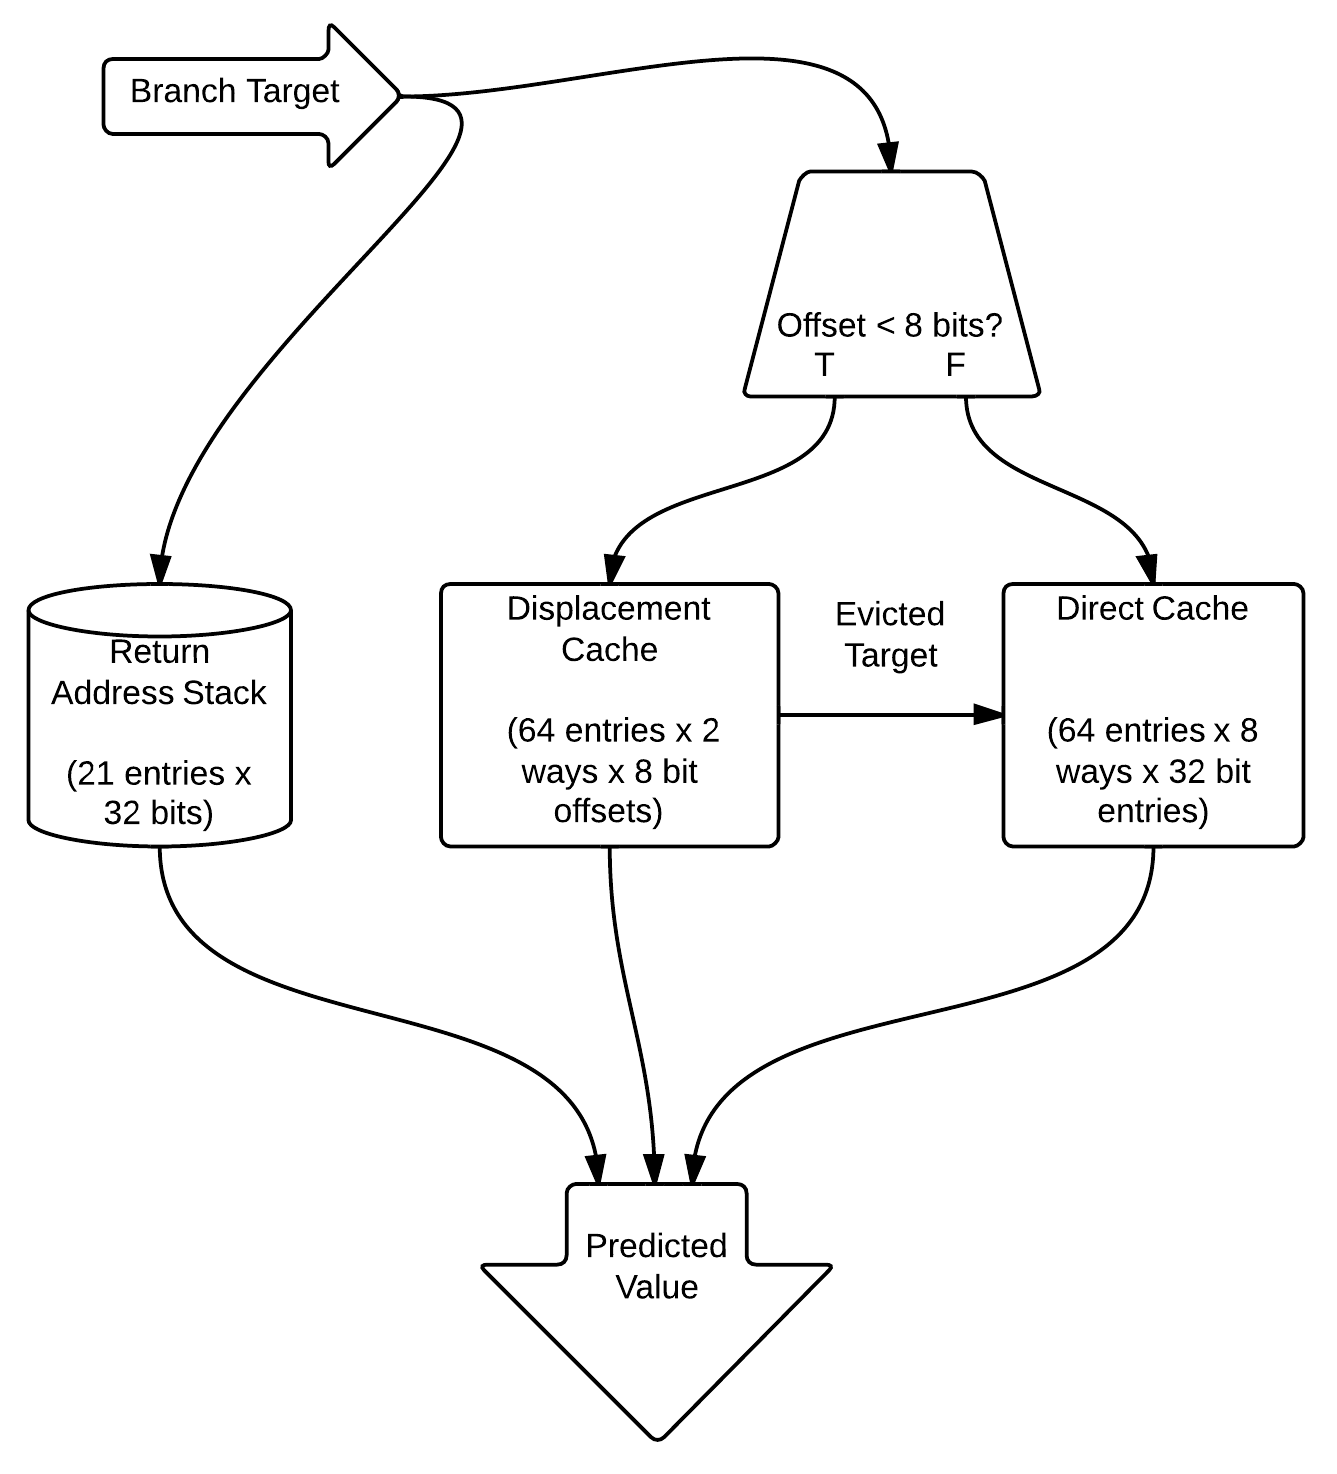
\includegraphics[width=\columnwidth]{BTB.png}}{Branch
  Target Predictor}{btbshape}

The branch target predictor also contains a return address stack. This
stack stores the return address of the last 21 calls. This allows
return addresses to be predicted, regardless of whether or not they
are in the cache. In addition to storing return addresses in the RAS,
return addresses are also placed in the displacement and direct
caches. 

\section{Implementation Details}
In order to determine the optimal cache design, the cache design was
generalized so that 


\section{Testing Methodology}
\centerimage{\includegraphics[width=\columnwidth]{random.pdf}}{Bitchin'
  Graph}{bgraph}
%Oracle predictor and BTB variables
%Table comparing Faust results to our results for Alpha
\section{Results}
%Table with all prediction rates for all tests
\section{Conclusion}
\newpage
\onecolumn
\section{Predictor.cc}
\lstinputlisting{../predictor.cc}[language=C++, showstringspaces=false]
\end{document}

